\chapter{Introduction}
Welcome to your remote lab for ECE/SE 380, Introduction to Feedback Control.
The lab portion of this course was designed to give you a hands-on
feel for control using analog circuits. Given the current climate, this is
clearly not possible in the way previously envisioned.

We persist. This lab is designed to run in MATLAB and Simulink. You will engage
in understanding, developing, executing and analyzing Simulink
diagrams that model and simulate control systems. Every lab is
provided with brief motivation on how one can see this applied in a real
world problem. I hope I can help connect the abstract block diagrams of
Simulink with the real world for you.

Control systems is a very broad topic with a long history that even predates
the ideas discussed in this course. This course and lab covers the very basic
notion of control, the idea of the negative feedback loop, buttressed by
the mathematical tools of linear dynamical systems.

\section{MATLAB and Simulink}
MATLAB is a desktop numerical and symbolic
mathematics computing environment. We will not rely heavily on MATLAB
scripting itself and instead use Simulink but you should be familiar with
both environments. Please ensure that, when you are installing MATLAB, you
install
%
\begin{enumerate}[label=(\arabic*)]
  \item{
    MATLAB,
  }
  \item{
    Simulink,
  }
  \item{
    the Control Systems Toolbox,
  }
  \item{
    the Simulink Control Design,
  }
  \item{
    the DSP System Toolbox,
  }
  \item{
    the Signal Processing Toolbox,
  }
  \item{
    the Statistics and Machine Learning Toolbox and
  }
  \item{
    the Symbolic Math Toolbox.
  }
\end{enumerate}
%
Simulink is an add-on to MATLAB that allows you to design and simulate
systems (physical or otherwise) using block diagrams like in
Figure~\ref{fig:intro:1}.
%
\begin{figure}[H]
  \centering
  \begin{tikzpicture}[x=1in, y=1in]
    \node [draw, block] (Controller) {\(K_p + K_i\frac{1}{s}\)};
    \node [draw, block, right=0.5 of Controller] (Plant) {\(\frac{1}{s}\)};
    \node [draw, summer, left=0.5 of Controller] (Sum) {};
    \node [below=0.5 of Sum] (BelowSum) {};

    \draw [arrow, signal]
      (Controller.east) -- (Plant.west);
    \draw [arrow, signal]
      (Plant.east)
      --
      +(0.35, 0)
      |-
      (BelowSum.base)
      --
      (Sum.south)
      node [below right, annotate] {\(-\)};
    \draw [arrow, signal]
      (Sum.east) -- (Controller.west);
    \draw [arrow, signal]
      ($(Sum.west)+1*(-0.5, 0)$) -- (Sum.west);
    \draw [arrow, signal]
      (Plant.east) -- +(0.7, 0);
  \end{tikzpicture}
  \caption[Example Feedback Diagram]{
    Example feedback diagram. The blocks are differential equations, expressed
    as a Laplace transfer function, that take an input signal and produce an
    output signal.
  }
  \label{fig:intro:1}
\end{figure}
%
Figure~\ref{fig:intro:1} can be replicated perfectly in Simulink.
That fact makes it easy for engineers to quickly design and verify
control designs. Simulink even supports direct interaction with
hardware but we will not utilize this feature.

The core of Simulink is the notion of a \emph{block}, maps that take an input
signal and produce an output signal.
The blocks we'll be concerned with primarily are \emph{gains}
(multiplier) depicted in Simulink like
\begin{center}
  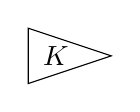
\begin{tikzpicture}[x=1em, y=1em]

    \draw
      (0, 0)
      --
      (3, 1)
      --
      (0, 2)
      --
      (0, 0)
      --
      (3, 1)
      node [at={(1, 1)}] {\(K\)};

  \end{tikzpicture}
\end{center}
and \emph{transfer functions} depicted in Simulink like
\begin{center}
  \begin{tikzpicture}[x=1em, y=1em]

    \node [draw, block] (Plant) {\(\frac{s+1}{s+2}\)};

  \end{tikzpicture}.
\end{center}
You may be provided template blocks to help you setup the Lab plant, the
system we wish to control; it will then be your task to analyze this block,
design a controller, and implement it by linking up blocks
in the appropriate feedback architecture.

\section{Lab Logistics and Deliverables}\label{intro:logistics}
Lab deadlines can be found in your course outline and on LEARN.
Read carefully.
Times are provided in the active Eastern Time.
Every lab requires you to complete a number of procedures described in green boxes like
\begin{procedure}[]
  Here are some steps:
  \begin{enumerate}[label=(\arabic*)]
    \item{Yes here is step 1,}
    \item{oh wow step 2,}
    \item{you got the idea.}
  \end{enumerate}
\end{procedure}
\noindent
and deliverables described in red boxes like
\begin{deliverable}[]
  Here are some things you will need to save for your report.
\end{deliverable}
Procedures are simply steps you should follow that will eventually result in one or more deliverables, namely something you must record and submit as part of your report. {\color{red}Note that the sequential number of the procedure may differ from the number of the deliverable. Procedures are, nevertheless, positioned and numbered such that they integrate well in the flow of information of specific sections. In other words, do not skip content trying to jump from a deliverable to what you may think is the corresponding procedure simply based on the procedure's number.}\\

Every lab chapter ends with a final summative deliverable, usually
consisting of a series of questions that you must answer.
%
All the deliverables should be packaged up in an organized way; ideally
they should be in your report in the order presented under headings directly corresponding to the deliverable label (1.1, 1.2, etc.). \\

We expect that the majority of your submissions will be typeset. However, for parts that involve a lot of formulas/diagrams/equations, it is acceptable to include \textbf {neatly hand-written parts}; make sure that they are \textbf {organized and legible}.
Your final report must be submitted as one PDF document on Learn; it is the duty of both lab partners to verify that the PDF file has been rendered correctly.
Your grade is entirely based on your report.\\

Occasionally, there has been confusion about what is allowed and what is not allowed in labs. You are responsible for knowing what constitutes an "academic offence" according to \href{https://uwaterloo.ca/secretariat/policies-procedures-guidelines/policy-71} {Policy 71} of the university. In particular, according to this policy:
\begin{enumerate}
\item{Cheating is an academic offence. Cheating includes copying from another student's work or allowing another student to copy from one's own work, submitting another person's work as one's own, fabrication of data and use of unauthorized aids.}
\item{Plagiarism (the act of presenting the ideas, words, or other intellectual property of another as one's own) is an academic offence. The use of other people's work must be completely and unambiguously acknowledged and referenced in all written material, including laboratory reports and computer programs.}
\end{enumerate}

In this course, labs are being done in groups of two students, subject to enrolment constraints. Each group must do their own analysis and their own design, do their own edits to the Matlab/Simulink files provided, and write up their own lab report. However:
\begin{enumerate}
\item{You may talk to the lab instructor, the teaching assistant and the course instructor about any aspect of the lab.}
\item{You are allowed to consult with other students in the class or share \emph{high-level ideas and approaches}, but \emph{not} to share detailed analysis or detailed design results.}
\item{You may not obtain or look at lab reports (either in hardcopy or softcopy) written by other students, whether they are current students or former students of ECE/SE 380. You may not let any other student access any part of your lab report (either in hardcopy or softcopy).}
\item{In your report, you must completely and unambiguously acknowledge and reference any person, website, report, book, or notes that you used to help you with your work. You should reference this lab manual, and the course notes, for example.}
\item{You must include in each report, and sign, the following statement:}
\end{enumerate}

\begin {declaration} \label{intro:decl} \hypertarget{intro:decl}
  We acknowledge and promise that: 
  \begin{enumerate}[label=\emph{\alph*})]
  \item We are the sole authors of this lab report and associated simulation files/code.
  \item This work represents our original work.
  \item We have not shared detailed analysis or detailed design results, computer code, or Simulink diagrams with any other student.
  \item We have not obtained or looked at lab reports from any other current or former student of ECE/SE 380, and we have not let any other student access any part of our lab work.
  \item We have completely and unambiguously acknowledged and referenced all persons and aids used to help us with our work.
  \end{enumerate}
  Student1 Name and Signature:\\
  Student2 Name and Signature: 
\end{declaration}

Every lab has its own grading scheme, but the following penalties apply equally to all labs:
\begin{itemize}
  \item{
    \(-5\%\) for poor organization or hand-written parts that are messy or difficult to read,
  }
  \item{
    \(-5\%\) for the submission not being in PDF format,
  }
  \item{
  	\(-5\%\) for not including the \hyperlink{intro:decl}{Declaration of Authorship} shown above,}
  \item{
    \(-1\%\) per hour within the first 24 hours past the submission deadline. After 24 hours, the penalty becomes \(-100\%\). If prior arrangements are made or a valid reason presented within one week from the missed deadline, the late penalty is waived. In no case will a lab report be accepted more than one week past the deadline. If a valid reason exists for being unable to hand in the lab report
    within the week following the deadline, then a solution tailored to each particular situation will be offered.  \textbf{Contact the Lab Instructor for this.}
    All reports are due at \texttt{23:59 Eastern Time} on the due date shown in the Course Outline.
   }
\end{itemize}
Minor mistakes are penalized quite steeply so check your work.
Mistakes in discussions usually amount to theoretical mistakes in understanding;
we will make an attempt to avoid double, or any other cascade, deduction.
